
\section{Modelagem pelo Método dos Elementos Finitos}

Em posse de \eqref{eq:edp_geomec_contorno}, é necessário um método numérico para encontrar sua solução. O método utilizado nesse trabalho é o dos Elementos Finitos que irá transformar  \eqref{eq:edp_geomec_contorno} em um sistema linear. De acordo com \cite{jacob}, o método dos Elementos finitos é bastante difundido, ele é utilizado em análise de tensões, transferência de calor, escoamento de fluido e eletromagnetismo. Em particular, a parte de análise de tensões e escoamento de fluído são importantes para a Engenharia de Reservatórios.



\subsection{Formulação Fraca}

O primeiro passo para utilizar o método dos elementos finitos é chegar na formulação fraca de \eqref{eq:edp_geomec_contorno}. As referências \cite{hughes} e \cite{jacob} mostram a dedução para chegar em \eqref{eq:weakform} e provam também a equivalência dela para a forma original (chamada de forma forte) com exceção do termo relacionado à pressão de poros, pois tratam do problema clássico de elasticidade linear. A forma fraca com esse termo pode ser encontrado em \citet{femgeomec}. A notação utilizada aqui é baseada em \cite{casteletto}, para manter a coerência com o Capítulo \ref{ch:multiescala}.


\begin{empheq}[box=\mymath]{equation}\label{eq:weakform}
\begin{split}
\text{Encontrar  }  \mathbf{u} \in \test \text{ tal que} \qquad \qquad \qquad \qquad \qquad \qquad \qquad \qquad \\
\omeint{ (\sopnabla \mathbf{w})^T \mathbf{D} \sopnabla  \mathbf{u}} - \int_{\Gamma_\sigma} \mathbf{w}^T \bar{\mathbf{t}} d\Gamma = (\sopnabla\mathbf{w})^T \mathbf{m} P_p \quad \forall \mathbf{w} \in \trial
\end{split}
\end{empheq}



Com conjunto de teste $\trial = \trialdef$ e conjunto de avaliação igual a $\test = \testdef$. Onde $\sobolev$ representa o espaço de Solobev de grau um.

\subsection{Divisão do domínio}

O domínio do problema será dividido em uma quantidade finita de elementos, o conjunto desses elementos será chamado de $\tau^h$.  A partição do domínio será realizada em elementos quadriláteros e seus vértices são denominados nós. A Figura \ref{fig:elemento} mostra um exemplo dessa divisão para um determinado domínio.

%TODO trocar por figura em que os elementos não sejam
\begin{figure}[!htbp]
\centering
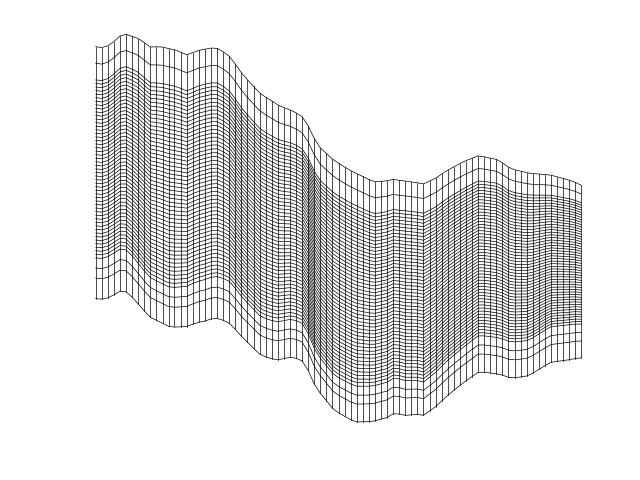
\includegraphics[width=0.8\textwidth]{chap01/figs/exemplo_dominio.png}
\caption{Exemplo de domínio/reservatório dividido em quadriláteros.}
\label{fig:elemento}
\end{figure}


Dadas a forma fraca definida em \eqref{eq:weakform} e funções de forma $\basefunctionfine$ para $i = 1, 2, 3, ..., \qtdfreedomfine + \qtdessentialfine$, pode-se encontrar uma solução aproximada pelo método de elementos finitos de Galerkin. Onde $\qtdfreedomfine$ representa a quantidade de graus de liberdade e $\qtdessentialfine$ está relacionado com os graus de liberdade que caíram em condições de contorno de Dirichlet. O método consiste em procurar solução não mais para $\mathbf{w} \in \trial$ e $\mathbf{u} \in \test$, mas em encontrar uma solução aproximada onde  $\mathbf{w^h} \in \trialaprox = \text{span}\{ \basefunctionfine | i = 1,2, ..., \qtdfreedomfine  \}$ e $\mathbf{u}$ é  da forma aproximada mostrada em \eqref{eq:udiscret}. 

\begin{equation}\label{eq:udiscret}
\mathbf{u}(\mathbf{x}) = \sum_{i=1}^{\qtdfreedomfine} \basefunctionfine  d_i^h + {\sum_{i=1}^ {n^h_{\bar{u}}}}  \basefunctionfineessential \bar{d}_i^h
\end{equation}



Onde cada $d_i^h$ representa um grau de liberdade associado a um nó que, a princípio, tem dois graus de liberdade, um para a direção x e outro para a direção y, a menos dos nós que estão em fronteiras com condição de contorno de Dirichlet. Nesse caso, os nós terão associados valores $\bar{d}_i^h$  iguais ao valor especificado pela condição para garantir que elas sejam satisfeitas. É importante perceber que, com essas aproximações, a busca da solução está sendo realizada em espaços de dimensão finita, diferentemente da forma fraca original onde os espaços $\trial$ e $\test$ são infinitos.


Com isso pode-se chegar na forma fraca aproximada \eqref{eq:weakformaprox}. Caso a solução do problema original pertença a $\trialaprox$ a solução exata ainda será encontrada pelo método.

\begin{equation}\label{eq:weakformaprox}
\omeint{ (\sopnabla \mathbf{w}^h)^T \mathbf{D} \sopnabla  \mathbf{u}^h}  =  \int_{\Gamma_\sigma} \mathbf{w}^{h^T} \bar{\mathbf{t}} d\Gamma  +  \omeint{(\sopnabla\mathbf{w}^h)^T \mathbf{m} P_p}  \quad \forall \mathbf{w}^{h^T} \in \trialaprox
\end{equation}


 %Para esse tipo de elemento a quantidade de vértices é quatro. Como o campo aproximado de deslocamentos está no plano xy, cada vértice terá dois graus de liberdade um na direção x e um na direção y, que de maneira indistinta serão chamados de $d_i^h$ para algum $i$ que são as variáveis a serem descobertas para encontrar a solução $\textbf{u}$ aproximada. A quantidade de graus de liberdade será chamada de $\qtdfreedomfine$. Um nó pertencente a fronteira de $\Omega$  já tem seu grau de liberdade determinado e, portanto, não será uma variável do problema e esses valores serão chamados de $\bar{d}_i^h$ a quantidade de graus de liberdade pertencentes a fronteira de dirichlet será chamada de $\qtdessentialfine$.  Assim, o campo vetorial $u$ será aproximado através de funções $ \basefunctionfine : \Omega \rightarrow \mathbb{R}^2 \quad \forall \quad i=1,2,...,\qtdfreedomfine$  relativa aos graus de liberdade e  $ \basefunctionfine : \Omega \rightarrow \mathbb{R}^2 \quad \forall \quad i=\qtdfreedomfine+1,2,...,\qtdfreedomfine + \qtdessentialfine$  relativas as condições de contorno de Dirichlet através de \eqref{eq:udiscret}.


A Equação \eqref{eq:udiscret} também pode ser reescrita utilizando vetores,

\begin{equation}\label{eq:udiscretvetor}
\mathbf{u}(\mathbf{x}) = \mathbf{N^h} \mathbf{d}^h + \mathbf{\bar{N}^h} \mathbf{\bar{d}}^h
\end{equation}

onde

\begin{eqnarray*}
\mathbf{N^h} = [N^h_1, N^h_2, ..., N^h_{\qtdfreedomfine} ] \\
\mathbf{\bar{N}^h}  =[N^h_{\qtdfreedomfine + 1}, N^h_{\qtdfreedomfine + 2}, ..., N^h_{\qtdfreedomfine + \qtdessentialfine}] \\
\mathbf{d} = [d_1^h, d_2^h, ... , d_{\qtdfreedomfine}^h]^T \\
\bar{\mathbf{d}} = [\bar{d}_1^h, \bar{d}_2^h, ... , \bar{d}_{\qtdessentialfine}^h]^T
\end{eqnarray*}

\suge{explicar o que significam os índices em  $\qtdfreedomfine$}

As funções $\basefunctionfine: \Omega \rightarrow \mathbb{R}^2$, em uma abordagem clássica de elementos finitos, são da forma $[N^h_{i_x} \quad 0]^T$ para um grau de liberdade x e  $[0 \quad N^h_{i_y}]^T$  para um grau de liberdade y, portanto, um grau de liberdade x não é utilizado para interpolar o valor do campo $u_y(x, y)$ e vice-versa. Além disso, para um nó com  graus de liberdade $d^h_i$ para x e $d^h_j$ para y, tem-se $N^h_{i_x} = N^h_{j_y}$ que, de acordo com \cite{jacob} é a forma mais usual. \suge{explicar o que significam os índices em  $N^h_{j_y}$}
As funções $N^h_{i_x}$  e $N^h_{j_y}$ são tais que assumem valor um no seu nó correspondente e possuem valor zero em todos os outros nós, mais especificamente, o suporte dessas funções são apenas os elementos que possuem o nó correspondente como vértice e são bilineares em cada um desses elementos (bilineares por partes). A Figura \ref{fig:grid3x3ver} mostra a numeração dos nós em uma malha 3x3 enquanto a Figura \ref{fig:numeracaofuncoes} apresenta a numeração das funções $\basefunctionfine$ considerando condições de Dirichlet na borda inferior.
Exemplos das funções são apresentadas na Figura \ref{fig:shapefunctions}.
Um detalhe importante é que as funções de forma que serão utilizadas no método multiescala, apresentadas no Capítulo \ref{ch:multiescala}, não possuem a propriedade de uma de suas componentes ser nula.


\begin{figure}[h]
\center
\subfigure[ Numeração global dos nós em malha $3\times3$. Marcados de vermelho o nó 6 e seus adjacentes. ]{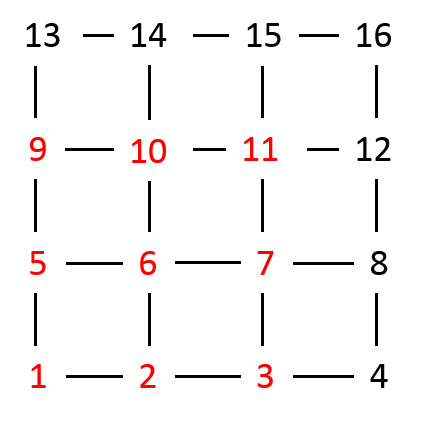
\includegraphics[width=0.40\textwidth]{chap01/figs/grid3x3ver.png}\label{fig:grid3x3ver}}
\qquad
\subfigure[ Numeração das funções de forma $N_i^h$. Azul as funções de forma relativa à condição de contorno de Dirichlet ]{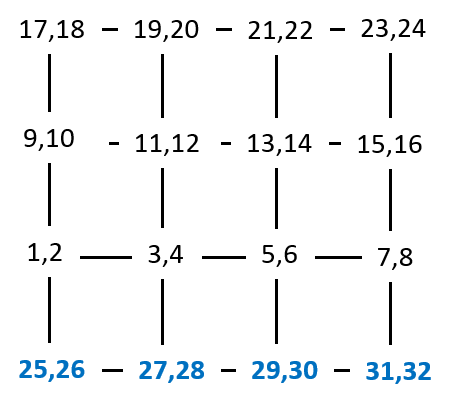
\includegraphics[width=0.45\textwidth]{chap01/figs/grid3x3_Ni.png}\label{fig:numeracaofuncoes}}

\caption{Numeração dos nós e das funções de base. Para numeração das funções de base foi considerada a borda inferior com condição de Dirichlet nas direções x e y. }
\end{figure}


\begin{figure}[h]
\center
\subfigure[ ${\basefunctionfine[9x]}$ ou ${\basefunctionfine[10y]}$ ]{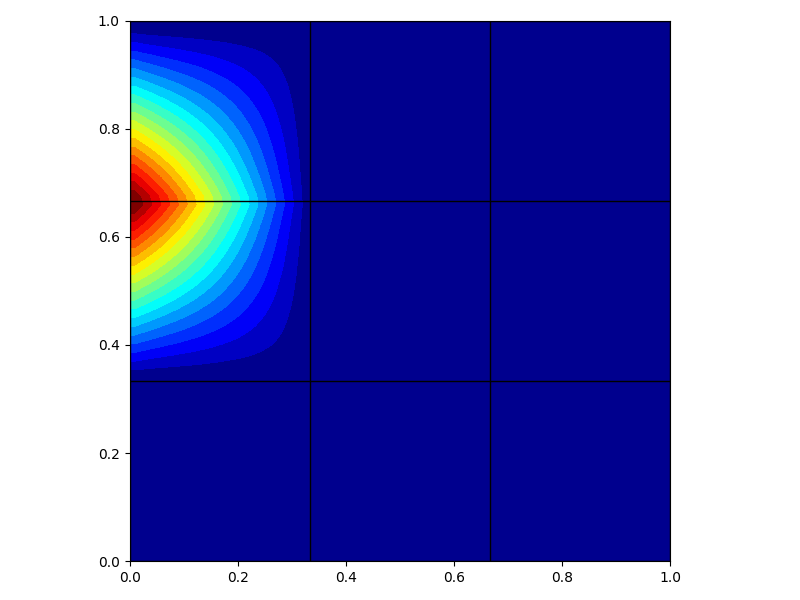
\includegraphics[width=0.45\textwidth]{chap01/figs/prolongation/prolongation_x_total_016.png}}
\qquad
\subfigure[ ${\basefunctionfine[13x]}$ ou ${\basefunctionfine[14y]}$ ]{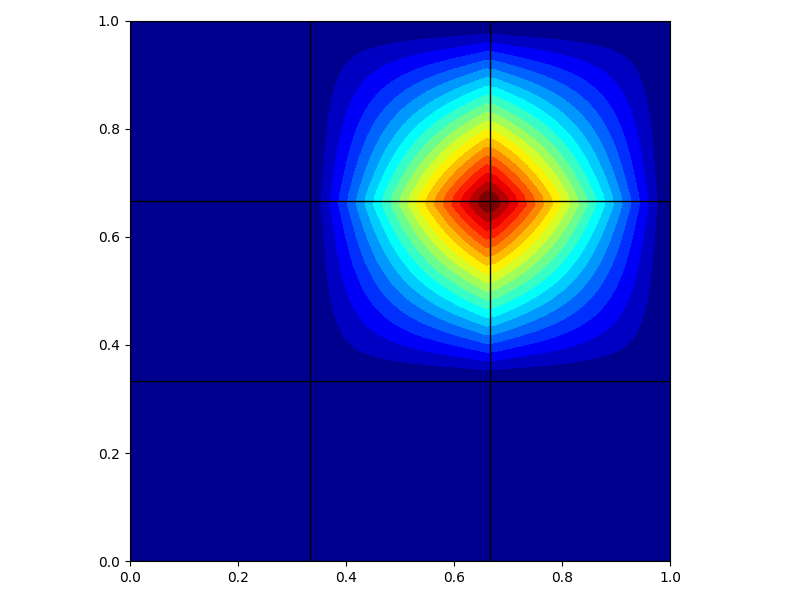
\includegraphics[width=0.45\textwidth]{chap01/figs/prolongation/prolongation_x_total_020.png}}

\subfigure[ ${\basefunctionfine[27x]}$ ou ${\basefunctionfine[28y]}$ ]{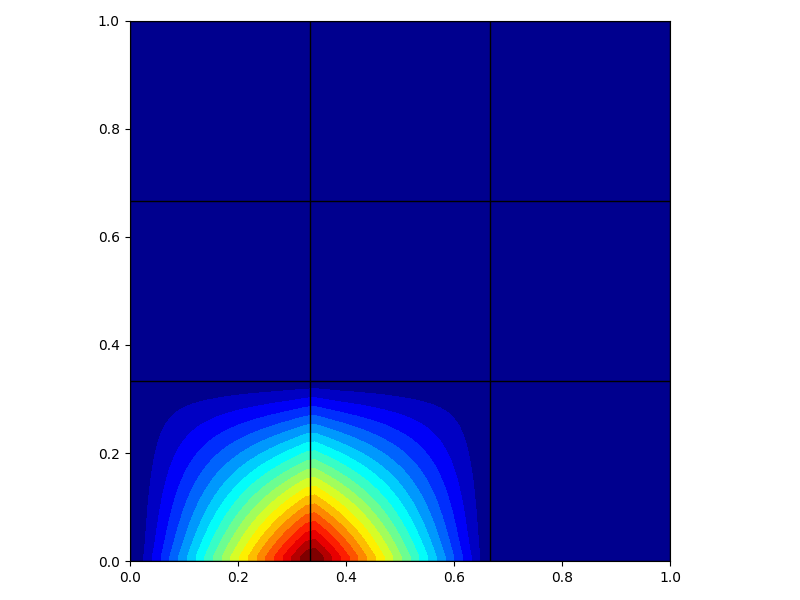
\includegraphics[width=0.45\textwidth]{chap01/figs/prolongation/prolongation_x_total_002.png}}
\qquad
\subfigure[ ${\basefunctionfine[31x]}$ ou ${\basefunctionfine[32y]}$ ]{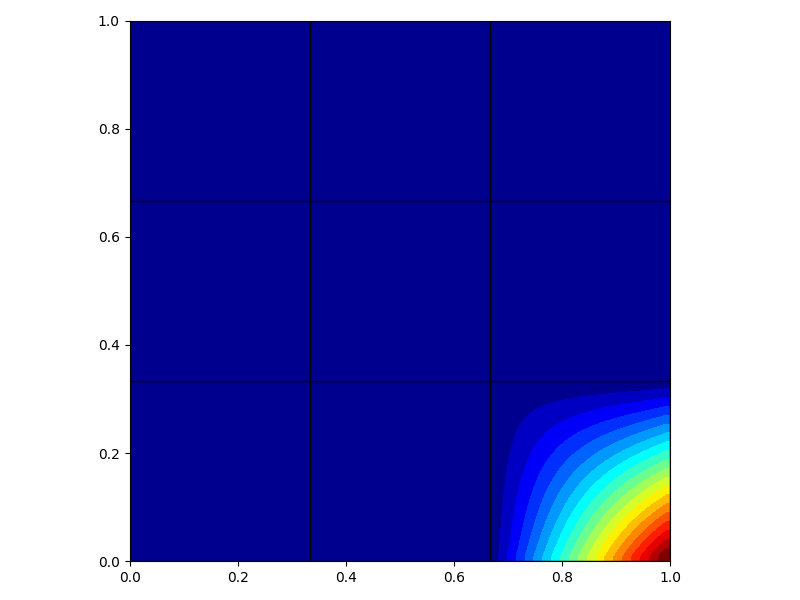
\includegraphics[width=0.45\textwidth]{chap01/figs/prolongation/prolongation_x_total_006.png}}
\caption{Gráficos das funções de forma para um grid 3x3. Foi considerada a mesma numeração apresentada na Figura \ref{fig:numeracaofuncoes}. }\label{fig:shapefunctions}
\end{figure}



\subsection{Construção do sistema linear}

É importante perceber que as variáveis a serem descobertas são as do vetor $\mathbf{d}^h$, dado que as entradas de $\mathbf{\bar{d}}^h$ já estão definidas pelos valores da fronteira. Os valores de $\mathbf{d}^h$ são encontrados a partir da solução de um sistema linear.

Para obter um sistema linear, pode-se substituir $\mathbf{w}^h$ por cada uma das funções $\basefunctionfine$ para $i = 1, 2, 3, ..., \qtdfreedomfine$ em \eqref{eq:weakformaprox}. Seguem abaixo os cálculos substituindo $\mathbf{w}^h$ por $\basefunctionfine$ e $\mathbf{u}^h$ por \eqref{eq:udiscretvetor}.


\begin{equation}
\omeint{ (\sopnabla \basefunctionfine)^T \mathbf{D}\sopnabla (\mathbf{N^h} \mathbf{d}^h + \mathbf{\bar{N}^h} \mathbf{\bar{d}}^h )} = \neumann + \poroload
\end{equation}

\begin{equation*}
\omeint{ (\sopnabla \basefunctionfine)^T \mathbf{D}\sopnabla \mathbf{N^h} \mathbf{d}^h }  = \neumann + \poroload - \omeint{ (\sopnabla \basefunctionfine)^T \mathbf{D}\sopnabla  \mathbf{\bar{N}^h} \mathbf{\bar{d}}^h}
\end{equation*}

\begin{equation}\label{eq:umaequacaosistema}
\omeint{ (\sopnabla \basefunctionfine)^T \mathbf{D}\sopnabla \mathbf{N^h}}  \mathbf{d}^h   = \neumann + \poroload - \omeint{ (\sopnabla \basefunctionfine)^T \mathbf{D}\sopnabla  \mathbf{\bar{N}^h} } \mathbf{\bar{d}}^h
\end{equation}


Definindo,

\begin{equation}\label{eq:entradamatriz}
    \rigidmatrixentry = \omeint{\kij{i}{j}} 
\end{equation}

e

\begin{equation}\label{eq:entradald}
    [\mathbf{f}^h]_i = \neumann + \poroload - \omeint{ (\sopnabla \basefunctionfine)^T D \sopnabla  \mathbf{\bar{N}^h} } \mathbf{\bar{d}}^h
\end{equation}



A parcela da integral do lado esquerdo pode ser reescrita como:

\begin{equation}
\omeint{(\sopnabla \basefunctionfine)^T \mathbf{D} \sopnabla \mathbf{N^h} }= [ [\rigidmatrix]_{i,1}\quad   [\rigidmatrix]_{i,2} \quad ... \quad  [\rigidmatrix]_{i,\qtdfreedomfine}] =  [\rigidmatrix]_{i,:}
\end{equation}

e então chegar em \eqref{eq:umaequacaosistemafim}.

\begin{equation} \label{eq:umaequacaosistemafim}
[\rigidmatrix]_{i,:} \mathbf{d}^h = [\mathbf{f}^h]_i \quad \forall \quad i=1,..., \qtdfreedomfine
\end{equation}

Finalmente, substituindo  $i = 1, 2, ..., \qtdfreedomfine$ pode-se encontrar o sistema linear \eqref{eq:sistemalinear}.

\begin{equation}\label{eq:sistemalinear}
    \rigidmatrix \mathbf{d}^h = \mathbf{f}^h
\end{equation}
onde as entradas de $\rigidmatrix $ são definidas por \eqref{eq:entradamatriz}. A solução do sistema tem como resultado os valores de cada um dos graus de liberdade $\freedomfine$ e, portanto, é possível encontrar a aproximação dos deslocamentos com \eqref{eq:udiscret}. Sobre a matriz $\rigidmatrix$, ela satisfaz as seguintes propriedades:


\begin{itemize}
    \item A matriz é simétrica, pois:

    \begin{eqnarray}
    \rigidmatrixentry & = & (\rigidmatrixentry)^T \\
            & = & \omeint{((\sopnabla \basefunctionfine)^T D \sopnabla \basefunctionfine[j])^T} \\
            & = & \omeint{ ( \sopnabla \basefunctionfine[j])^T D^T  ((\sopnabla \basefunctionfine)^T)^T}\\
            & = & \omeint{ ( \sopnabla \basefunctionfine[j])^T D  (\sopnabla \basefunctionfine)} \\
            & = & [\rigidmatrix]_{j,i}
    \end{eqnarray}


    \item A matriz é esparsa. Pois cada uma das funções de forma é não nula apenas nos elementos em que aquele nó é vértice e, portanto, a intersecção dos suportes de $\basefunctionfine$ e $\basefunctionfine[j]$ é não vazia somente se estiverem associadas a vértices que estão um elemento em comum. No caso de uma malha de quadriláteros, cada função de forma é não nula em quatro elementos apenas.

    \item A matriz é positiva definida. A prova desse fato é encontrada em \cite{hughes}, que mostra que esse propriedade depende da relação constitutiva ser também positiva definida.
\end{itemize}


Ainda sobre a esparsidade da matriz de rigidez em um grid com quadriláteros, cada função de base de um nó (a menos de nós de fronteira) tem conexão com nove outros nós, contando com ele mesmo. Como mostra a Figura \ref{fig:grid3x3ver} o nó 6 tem conexões com os nós [1,2,3,5,6,7,9,10,11]. Considerando a simplificação que cada nó possui os dois graus de liberdade isso implica em duas linhas correspondentes na matriz de rigidez, e cada linha possui $2 \times 9 = 18$ valores não nulos, portanto, cada nó tem $2 \times 18 = 36$ não zeros associados na matriz, o que leva a uma aproximação para o número de não nulo da matriz de $\text{nnz}_{\rigidmatrix} = 36 \qtdnos$. Como será mostrado no Capítulo \ref{ch:sistemas}, a matriz terá que utilizar alguma estrutura de matriz esparsa, pois caso fosse alocada densa a quantidade de valores alocados seria aproximadamente $(2 \times \qtdnos)^2$ que tem ordem quadrática com o número de nós e limitaria rapidamente o tamanho dos modelos simulados.


Apesar de ter sido mostrado explicitamente quanto vale cada entrada em \eqref{eq:entradamatriz} a montagem da matriz não é feita dessa forma. As integrais que aparecem no domínio $\Omega$ serão divididas em cada um dos elementos passando da forma \eqref{eq:matrizrigidezaberta} para \eqref{eq:matrizrigidezporelemento}.


\begin{equation}\label{eq:matrizrigidezaberta}
\rigidmatrix  = \omeint{
\begin{bmatrix}
\kij{1}{1} & \kij{1}{2}  & \hdots & \kij{1}{\qtdfreedomfine} \\
\kij{2}{1} & \kij{2}{2}  & \hdots & \kij{2}{\qtdfreedomfine} \\
\vdots &  & \ddots & \vdots\\
\kij{\qtdfreedomfine}{1} & \kij{\qtdfreedomfine}{2}  & \hdots & \kij{\qtdfreedomfine}{\qtdfreedomfine}
\end{bmatrix}
}
\end{equation}


\begin{equation}\label{eq:matrizrigidezporelemento}
\rigidmatrix  = \sum_{e \in \tau^h} \omeeint{
\begin{bmatrix}
\kij{1}{1} & \kij{1}{2}  & \hdots & \kij{1}{\qtdfreedomfine} \\
\kij{2}{1} & \kij{2}{2}  & \hdots & \kij{2}{\qtdfreedomfine} \\
\vdots     &             & \ddots & \vdots\\
\kij{\qtdfreedomfine}{1} & \kij{\qtdfreedomfine}{2}  & \hdots & \kij{\qtdfreedomfine}{\qtdfreedomfine}
\end{bmatrix}
}
\end{equation}


Cada parcela da somatório dos elementos em \eqref{eq:matrizrigidezporelemento} é uma integral no domínio $\Omega^e$ de algum elemento e, portanto, apenas 8 funções de forma são não zero em $\Omega^e$. Então, apenas $8\times8=64$ valores são diferentes de zero em cada uma das matrizes do somatório. Assim, esse valores podem ser condensados em uma matriz menor $8\times8$ com uma numeração local do elemento conforme mostrado em \eqref{eq:matrizelementoraw}.

\begin{equation}\label{eq:matrizelementoraw}
\mathbf{K}^e =
\omeeint{
\begin{bmatrix}
\kije{1}{1} & \kije{1}{2}  & \hdots & \kije{1}{8}  \\
\kije{2}{1} & \kije{2}{2}  & \hdots & \kije{2}{8}  \\
\vdots      &              & \ddots & \vdots       \\
\kije{8}{1} & \kije{8}{2}  & \hdots & \kije{8}{8}
\end{bmatrix}
}
\end{equation}
Onde $\basefunctionelem[1], \hdots, \basefunctionelem[8]$ representam uma numeração local do elemento para as funções $\basefunctionfine$ que são não nulas nesse determinado elemento e $\mathbf{D}^e$ a matriz de elasticidade calculadas com as propriedades do elemento. E pode ser transformada em \eqref{eq:matrizelementosemiraw}.

\begin{equation}\label{eq:matrizelementosemiraw}
    \mathbf{K}^e =\omeeint{ (\sopnabla [\basefunctionelem[1] \basefunctionelem[2] \hdots \basefunctionelem[8] ]) ^T \mathbf{D} (\sopnabla [\basefunctionelem[1] \basefunctionelem[2] \hdots \basefunctionelem[8]])}
\end{equation}

Definindo,

\begin{equation}
    \mathbf{B}^e = \sopnabla [\basefunctionelem[1] \basefunctionelem[2] \hdots \basefunctionelem[8] ]
\end{equation}

A matriz de rigidez do elemento pode ser escrita como:

\begin{equation} \label{eq:matrizelemento}
    \mathbf{K}^e = \omeeint{(\mathbf{B}^e)^T \mathbf{D}^e \mathbf{B}^e}
\end{equation}


A montagem da matriz de rigidez pode ser feita calculando a matriz do elemento \eqref{eq:matrizelemento} e acumulando esses valores em suas respectivas posições globais. Abaixo, é apresentado  o algoritmo para montagem da matriz de rigidez global.

\vspace{1cm}
\begin{algorithm}[H]
\caption{MontagemMatrizRigidez}
\label{alg:buildmatrix}
\Inicio{

$\rigidmatrix \leftarrow \mathbf{0}$

\Para{\text{elemento} $e \in \tau^h$}{
    Calcule a matriz de rigidez do elemento $K^e$
    
    \Para{Grau de liberdade i em e}{
        \Para{Grau de liberdade j em e}{
            Acumule em $\rigidmatrix$ o valor  $K^e[i,j]$ na posição global correspondente
        }    
    }
}
}

\end{algorithm}
\vspace{1cm}



Algo que ainda precisa ser feito é mostrar como o cálculo da matriz $\mathbf{K}^e$ é realizado. O primeiro passo é modificar a integral para um domínio onde ela pode ser mais facilmente calculada, para isso, cada domínio $\Omega^e$ será associado a um elemento padrão  $\Omega^\xi = [-1,1]\times[-1,1]$ que é um elemento padrão em coordenadas $\xi$ e $\eta$. A Figura \ref{fig:bijecaoelemento} mostra a associação entre os dois elementos.


\begin{figure}[!htbp]
\centering
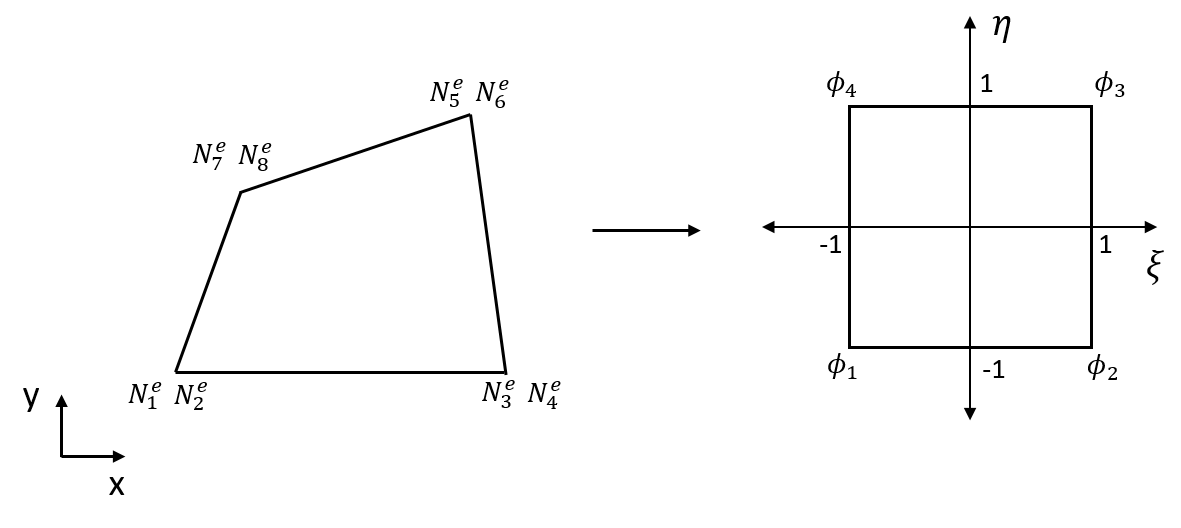
\includegraphics[height=6cm]{chap01/figs/elementopadrao.png}
\caption{Bijeção entre elemento $\Omega^e$ e $\Omega^\xi$}
\label{fig:bijecaoelemento}
\end{figure}


No elemento padrão $\Omega^\xi$ as funções de forma bilineares associadas aos nós são facilmente definidas como apresentado em \eqref{eq:definicaofuncform}.


\begin{equation}
\begin{matrix}\label{eq:definicaofuncform}
\phi_1(\xi, \eta) = \frac{1}{4} (1-\xi)(1-\eta) \\
\phi_2(\xi, \eta) = \frac{1}{4} (1-\xi)(1+\eta) \\
\phi_3(\xi, \eta) = \frac{1}{4} (1+\xi)(1+\eta) \\
\phi_4(\xi, \eta) = \frac{1}{4} (1+\xi)(1-\eta) \\
\end{matrix}
\end{equation}


Um ponto de $\Omega^e$ é associado a um ponto em $\Omega^\xi$ através de uma associação isoparamétrica de acordo com \eqref{eq:isoparametrico}.


\begin{equation}\label{eq:isoparametrico}
\begin{matrix}
x(\xi, \eta) = \sum_{A=1}^{4} \phi_A(\xi, \eta) x^e_A \\
y(\xi, \eta) = \sum_{A=1}^{4} \phi_A(\xi, \eta) y^e_A
\end{matrix}
\end{equation}

Onde $x^e_A$ e $y^e_A$ para $i=1,2,3,4$ são as coordenadas dos vértices do elemento.

Com isso, as funções $\phi$ em \eqref{eq:definicaofuncform} estão definidas implicitamente em função de x e y. As funções de base $\basefunctionfine$ assumem exatamente os valores dessas funções em um dado elemento. Portanto, pode-se reescrever a matriz $\bee$ da seguinte forma:


\begin{equation} \label{eq:bephi}
    \bee = \sopnabla \begin{bmatrix}
\phi_1 & 0      & \phi_2 & 0 & \phi_3 & 0 & \phi_4 & 0\\
0      & \phi_1 & 0 & \phi_2 & 0 & \phi_3 & 0 & \phi_4
\end{bmatrix}
\end{equation}


Assim é possível realizar uma substituição de variáveis na integral apresentada em \eqref{eq:matrizelementosemiraw}.


\begin{align}
\mathbf{K}^e      = & \omeeint{ (\bee)^T \mathbf{D}^e \bee} \nonumber \\
         = &  \intbase{ (\bee)^T \mathbf{D}^e \bee |\mathbf{J}|  }
\end{align}


Onde $\mathbf{J}$ representa o jacobiano

\begin{equation}
\mathbf{J} = \begin{bmatrix}
\dxi[x]   &  \dxi[y]    \\
\deta[x]  &  \deta[y]
\end{bmatrix}
\label{eq:jacobiano}
\end{equation}


A integral no domínio $[-1, 1] \times [-1,1] $ pode ser calculada através da Quadratura de Gauss que pode ser encontrado em \cite{jacob}. O método consiste em trocar a integral por um somatório ponderado por pesos $w_i$ em alguns pontos determinados da função, chamados de pontos de integração. A quantidade de pontos de integração determina quão boa é a aproximação para o caso. Com $n_p$ pontos de integração é possível integrar exatamente um
polinômio de tamanho $2n_p - 1$. % TODO adicionar tabela com pontos de integração?

Com isso a integral pode ser aproximada pelo somatório \eqref{eq:somatorioapprox}.

\begin{equation} \label{eq:somatorioapprox}
    \sum^{n_p}_{i=1} (\sopnabla [\basefunctionelem[1] \basefunctionelem[2] \hdots \basefunctionelem[8] ]) ^T \mathbf{D} (\sopnabla [\basefunctionelem[1] \basefunctionelem[2] \hdots \basefunctionelem[8]])|\mathbf{J}||_{x=p_i} w_i
\end{equation}

O cálculo do jacobiano em um determinado ponto pode ser calculado derivando  \eqref{eq:isoparametrico}

\begin{equation}\label{eq:jacobianoderivadas}
\begin{matrix}
\dxi[x] = \sum^4_{A=1} \dxi[\phi_A] x^e_A &  \deta[x] = \sum^4_{A=1} \deta[\phi_A] x^e_A\\
\dxi[y] = \sum^4_{A=1} \dxi[\phi_A] y^e_A &  \deta[y] = \sum^4_{A=1} \deta[\phi_A] y^e_A
\end{matrix}
\end{equation}


Além disso, para o cálculo de $\bee$ é necessário calcular as derivadas de $\phi_A$ em relação as coordenadas x e y.  Isso implica na inversão da matriz do Jacobiano, conforme mostrado abaixo.


\begin{equation}
\mathbf{J} \deriv = \der \rightarrow
\end{equation}

\begin{equation} \label{eq:devformglobal}
     \deriv = \mathbf{J} ^{-1}\der
\end{equation}

Com \eqref{eq:devformglobal}  é possível calcular as derivadas das funções de forma em função das coordenadas x e y. Feito isso, todos os termos da matriz $\bee$ podem ser obtidos finalizando assim o cálculo da matriz de rigidez do elemento.



\subsection{Cálculo da Carga por Diferença de pressão}

A Equação \eqref{eq:entradald}, mostra cada valor do vetor de carga $\mathbf{f}$. Três termos aparecem nesse caso: o primeiro relativo as condições de contorno de Neumann, o segundo relativo a pressão de poros e a terceira relativo as condições de contorno de Dirichlet. Nesse trabalho, o segundo termo será o de maior importância, pois serão calculados os deslocamentos no reservatório e rochas adjacentes em função de uma diferença de pressão causada pela produção do petróleo e/ou injeção de água. Devido a essas duas ações, a pressão de poros do reservatório irá variar gerando deformações e variação nas tensões da rocha.

Assim, o cálculo do lado direito será realizado através do somatório da contribuição de cada elemento análogo ao cálculo da matriz de rigidez. Abaixo, segue o cálculo da contribuição do elemento, será considerado que o campo de pressões será constante por elemento. Essa consideração foi realizada, pois esses valores serão recebidos de um simulador de fluxo que, geralmente, utilizam o método dos volumes finitos e, portanto, calculam as pressões nos elementos e não nos nós.

\begin{equation}
    \mathbf{f^e} = \omeeint{\begin{bmatrix}
(\sopnabla \basefunctionelem[1])^T \mathbf{m} \alpha^e P^e_p
\\
(\sopnabla \basefunctionelem[2])^T \mathbf{m} \alpha^e P^e_p
\\
(\sopnabla \basefunctionelem[3])^T \mathbf{m} \alpha^e P^e_p
\\
(\sopnabla \basefunctionelem[4])^T \mathbf{m} \alpha^e P^e_p
\\
(\sopnabla \basefunctionelem[5])^T \mathbf{m} \alpha^e P^e_p
\\
(\sopnabla \basefunctionelem[6])^T \mathbf{m} \alpha^e P^e_p
\\
(\sopnabla \basefunctionelem[7])^T \mathbf{m} \alpha^e P^e_p
\\
(\sopnabla \basefunctionelem[8])^T \mathbf{m} \alpha^e P^e_p
\end{bmatrix}},
\end{equation}
onde $\alpha^e$ e $P^e_p$ são os valores do coeficiente de Biot e de pressão do elemento \textit{e} em questão. Assim, pode-se continuar o calculo de $\mathbf{f^e}$.


\begin{equation}
\mathbf{f^e} = \omeeint{\begin{bmatrix}
(\sopnabla \basefunctionelem[1])^T
\\
(\sopnabla \basefunctionelem[2])^T
\\
(\sopnabla \basefunctionelem[3])^T
\\
(\sopnabla \basefunctionelem[4])^T
\\
(\sopnabla \basefunctionelem[5])^T
\\
(\sopnabla \basefunctionelem[6])^T
\\
(\sopnabla \basefunctionelem[7])^T
\\
(\sopnabla \basefunctionelem[8])^T
\end{bmatrix} \mathbf{m} \alpha^e P^e_p }
 = \omeeint{(\sopnabla  \begin{bmatrix} \basefunctionelem[1] & \basefunctionelem[2] & ... & \basefunctionelem[8]\end{bmatrix} )^T \mathbf{m}} \alpha^e P^e_p
\end{equation}

O primeiro termo da equação pode ser substituída por \eqref{eq:bephi}.


\begin{equation}
   \mathbf{ f^e } = \omeeint{(\sopnabla \begin{bmatrix}
                        \phi_1 & 0      & \phi_2 & 0 & \phi_3 & 0 & \phi_4 & 0\\
                        0      & \phi_1 & 0 & \phi_2 & 0 & \phi_3 & 0 & \phi_4
                    \end{bmatrix} ) ^ T \begin{bmatrix}
                    1\\1\\0
                    \end{bmatrix} \alpha^e P^e_p}
\end{equation}

\begin{equation} \label{eq:cargafinal}
   \mathbf{ f^e } = \omeeint{\begin{bmatrix}
    \dx[\phi_1] & 0           & \dy[\phi_1] \\
    0           & \dy[\phi_1] & \dx[\phi_1] \\
    \dx[\phi_2] & 0           & \dy[\phi_2] \\
    0           & \dy[\phi_2] & \dx[\phi_2] \\
    \vdots      & \vdots & \vdots      \\

    \dx[\phi_8] & 0           & \dy[\phi_8] \\
    0           & \dy[\phi_8] & \dx[\phi_8] \\

    \end{bmatrix} \begin{bmatrix}  1\\1\\0 \end{bmatrix} } \alpha^e P^e_p 
    = \omeeint{\begin{bmatrix}
      \dx[\phi_1] \\
      \dy[\phi_1] \\
      \dx[\phi_2] \\
      \dy[\phi_2] \\
      \vdots      \\
      \dx[\phi_8] \\
      \dy[\phi_8] \\
    \end{bmatrix} } \alpha^e P^e_p 
\end{equation}

A fórmula com a carga final utilizada é apresentada \eqref{eq:cargafinal}. Procedimento similar ao feito para a matriz de rigidez tem que ser feito para o cálculo dos valores: Mudança de variáveis para elemento padrão $\Omega^\xi$, substituição da integral por um somatório através da Quadratura de Gauss e cálculo da derivada das funções de forma no sistema de coordenadas x, y.


\subsection{Condições de Contorno}

As condições de contorno do problema já foram incorporadas no problema através do lado direito do sistema em \eqref{eq:entradald}, porém existem alternativas que, dependendo do caso, podem ser melhores para incorporar as condições de contorno ao problema. São apresentados aqui outras duas maneiras. As duas consistem de, ao invés de remover os graus de liberdade referentes as condições de Dirichlet,  adicioná-los na matriz de rigidez e forçar junto do lado direito que tenham o valor imposto pela condição de contorno. Com isso, a matriz de rigidez terá sempre o mesmo tamanho igual a $2\times \qtdnos$. A  \eqref{eq:bigconst} apresenta como a condição de contorno pode ser adicionada a matriz, onde o valor B representa um valor muito maior que os outros valores da linha.

\begin{equation} \label{eq:bigconst}
\begin{blockarray}{ccccc}
& \bar{d}_1^h &  & d_i ^h & & \\
& \downarrow &  & \downarrow & & \\
\begin{block}{c(cccc)}
\bar{d_1}^h \rightarrow & B & \hdots &  \kij{1+\qtdfreedomfine}{i}  & \hdots \\
\vdots                  &   & \vdots &             \\
d_i^h       \rightarrow &{ \color{red}\kij{i}{n_u^h + 1} }  &      & \kij{i}{i}   & \hdots \\
& \vdots &      & \vdots   &  \\
\end{block}
\end{blockarray} \begin{blockarray}{c}
 \\
 \\
\begin{block}{(c)}
\bar{d_1}^h \\
\vdots\\
d_i^h \\
\vdots  \\
\end{block}
\end{blockarray}\begin{blockarray}{c}
 \\
 \\
 \\
= \\
 \\
\end{blockarray} \begin{blockarray}{c}
 \\
 \\
\begin{block}{(c)}
 B \bar{u}_1 \\
\vdots\\
f^\prime_i \\
\vdots  \\
\end{block}
\end{blockarray}
\end{equation}
onde $\bar{u}_1$ representa o valor imposto pela condição de Dirichlet e $f^\prime_i$ representa o termo de \eqref{eq:entradald} sem o termo da condição de Dirichlet presente.

Dessa forma, a primeira equação quando resolvida mostra $B\bar{d}_1^h = B\bar{u}_1 \rightarrow \bar{d}_1^h = \bar{u}_1$, já a equação relativa ao grau de liberdade $d_i^h$ terá o lado direito $f^\prime_i$ complementada com o valor do lado esquerdo $\bar{d}_1^h \kij{i}{1+\qtdfreedomfine}$ (marcado em vermelho) ficando equivalente a \eqref{eq:entradald} novamente.

Uma variante dessa versão é zerar toda a linha relativa à $\bar{d}^h_1$ com exceção da diagonal principal que terá valor um, conforme mostrado em \eqref{eq:diagident}. Esse caso tem a desvantagem de remover a simetria da matriz.

\begin{equation} \label{eq:diagident}
\begin{blockarray}{ccccc}
& d_1^h &  & d_i ^h & & \\
& \downarrow &  & \downarrow & & \\
\begin{block}{c(cccc)}
\bar{d_1}^h \rightarrow & 1 & \hdots & 0 & \hdots \\
\vdots                  &   & \vdots &             \\
d_i^h       \rightarrow & \kij{i}{n_u^h + 1}   &      & \kij{i}{i}   & \hdots \\
& \vdots &      & \vdots   &  \\
\end{block}
\end{blockarray} \begin{blockarray}{c}
 \\
 \\
\begin{block}{(c)}
\bar{d_1}^h \\
\vdots\\
d_i^h \\
\vdots  \\
\end{block}
\end{blockarray} \begin{blockarray}{c}
 \\
 \\
 \\
= \\
 \\
\end{blockarray} \begin{blockarray}{c}
 \\
 \\
\begin{block}{(c)}
 \bar{u}_1 \\
\vdots\\
f^\prime_i \\
\vdots  \\
\end{block}
\end{blockarray}
\end{equation}


